\documentclass[a4paper,12pt, twoside, titlepage]{article}
\usepackage[utf8]{inputenc}
\usepackage{polski}
\usepackage[ddmmyyyy]{datetime}
\renewcommand{\dateseparator}{.}

\usepackage{lastpage}
\usepackage{fancyhdr}
\usepackage{graphicx}
\usepackage{hyperref}
\usepackage{longtable}
\usepackage{geometry}
\newgeometry{hmargin={20mm,20mm}, vmargin={30mm, 30mm}}


%\usepackage{hyperref}
%\hypersetup{
%    colorlinks,
%    citecolor=black,
%    filecolor=black,
%    linkcolor=black,
%    urlcolor=black
%}

%\renewcommand{\thesection}{\arabic{section}}

\pagestyle{fancy}
\fancyhf{}
\fancyhead[R]{\rightmark}
\fancyhead[L]{Eternal Fortification}
\fancyfoot[RO, LE]{\thepage \hspace{1pt} / \pageref{LastPage}}
\renewcommand{\footrulewidth}{0.5pt}

\renewcommand{\figurename}{Rysunek} 
\renewcommand{\sectionmark}[1]{\markright{#1}{}}

\title{\Huge{\textbf{Eternal Fortification}}\\ \Large{Projekt gry}\\ \large{Wersja 1.0}}
\author{Konrad Magiera}
\date{\today}


\begin{document}
\pagenumbering{gobble}
\maketitle
\newpage
\pagenumbering{arabic}
\tableofcontents
\newpage


\section{Przegląd}
\subsection{Gatunek}
Jest to strategiczna gra czasu rzeczywistego - Tower defense.

\subsection{Temat przewodni}
Gra porusza temat ewolucji, rozwoju cywilizacji. Kolejne poziomy wprowadzają gracza w następujące po sobie okresy rozwoju ludzkości.

\subsection{Opis projektu}


\subsection{Co wyróżnia projekt}
Pośród innych tytułów z gatunku Tower defense, Eternal Fortification wyróżnia motyw edukacyjny. Gra pozwala zapoznać się z uzbrojeniem wykorzystywanym przez ludzi na przestrzeni wieków.

\subsection{Dla kogo}
Idealnym odbiorcą będzie:
\begin{itemize}
	\item Osoba płci męskiej,
	\item Pasjonat historii,
	\item Osoba w wieku 15 - 24 lat.
\end{itemize}

\subsection{Użyta technologia}
Do stworzenia gry użyty zostanie silnik Unity3D oraz język C\#. Modele przygotowane zostaną w darmowym oprogramowaniu Blender.

\subsection{Wymagania systemowe}
\begin{itemize}
	\item System operacyjny: Windows 7/8.1.10,
	\item 1GB wolnego miejsca na dysku,
	\item 1GB RAM
\end{itemize}


\newpage
\section{Rozgrywka}
\subsection{Cel gry}
Gracz na każdym poziomie musi bronić się przed falami przeciwników. Warunkiem zwycięstwa jest przetrwanie określonej liczby fal dla danego poziomu. Liczba fal będzie różnić się pomiędzy poziomami podczas postępu w grze. Gracz przegrywa dany poziom gdy straci całe życia. Życia traci się gdy przeciwnicy dotrą do końca planszy.

\subsection{Tryb gry}

\subsubsection{Kampania}
Gracz z każdym zwycięstwem odblokowuje kolejne poziomy. W szczególnym przypadku odblokowana zostaje kolejna epoka, jeżeli wszystkie poziomy z danego okresu historycznego zostały ukończone. Kampania przenosi gracza w czasie, odkrywając kolejne okresy.

\subsection{Własny}
W tym trybie gracz buduje własne pole gry. Oprócz tego będzie możliwy wybór epoki osobno dla wież oraz przeciwników. Ten tryb zostanie odblokowany po przejściu pierwszej epoki w trybie kampania.


\subsection{Gracz}
\subsubsection{Sterowanie}
%\begin{figure}[!htb]
%		\begin{center}
%			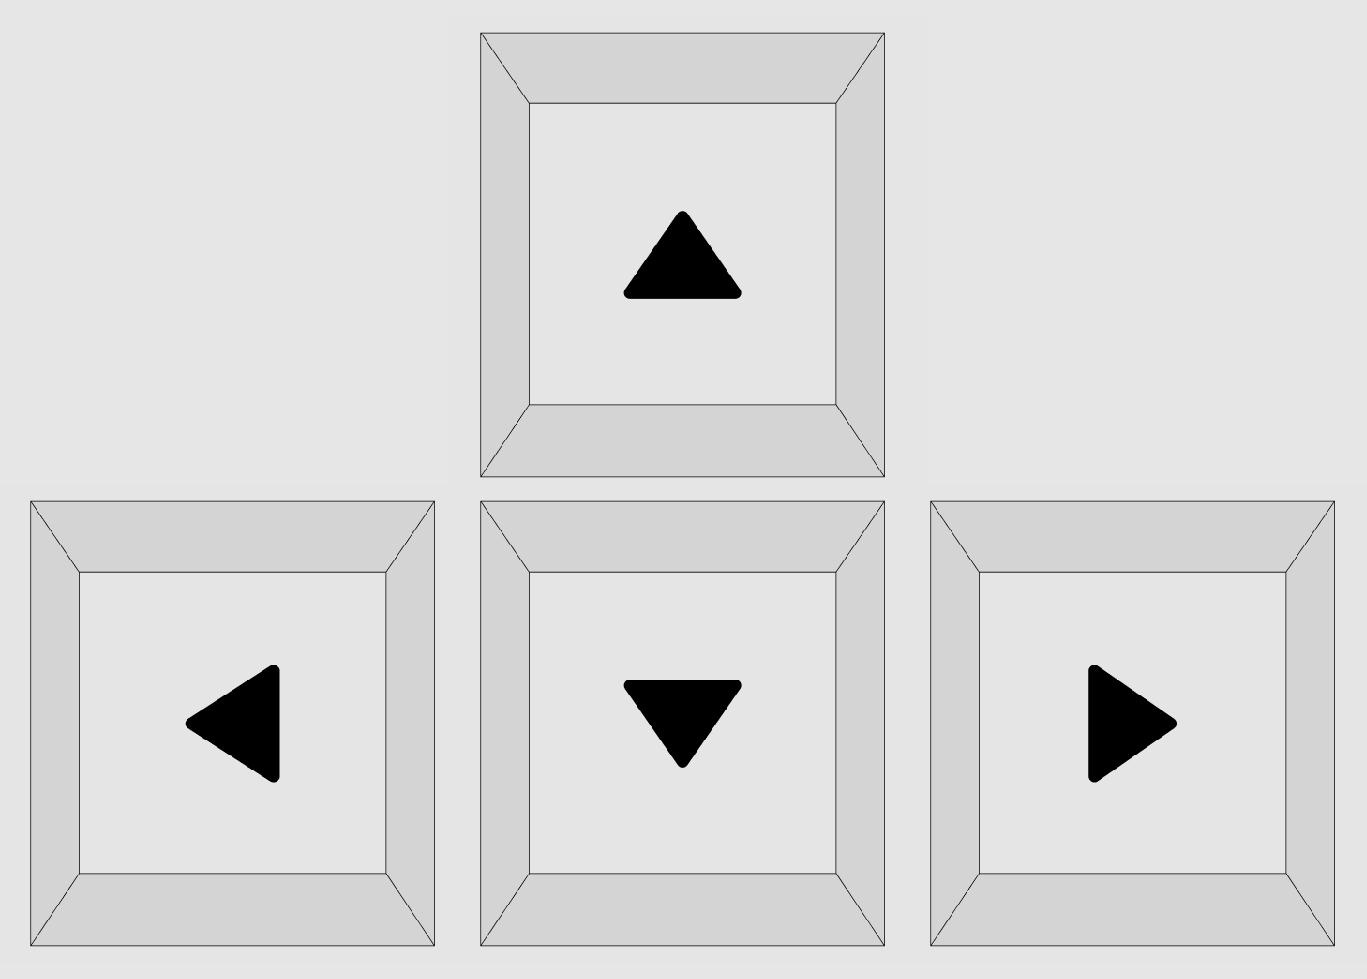
\includegraphics[height=3cm]{import/arrows.pdf}
%		\end{center}
%		\caption{Sterowanie}
%	\end{figure}

\begin{center}
\begin{longtable}{| p{.50\textwidth} | p{.50\textwidth} |} 
	\hline
	\begin{center}
		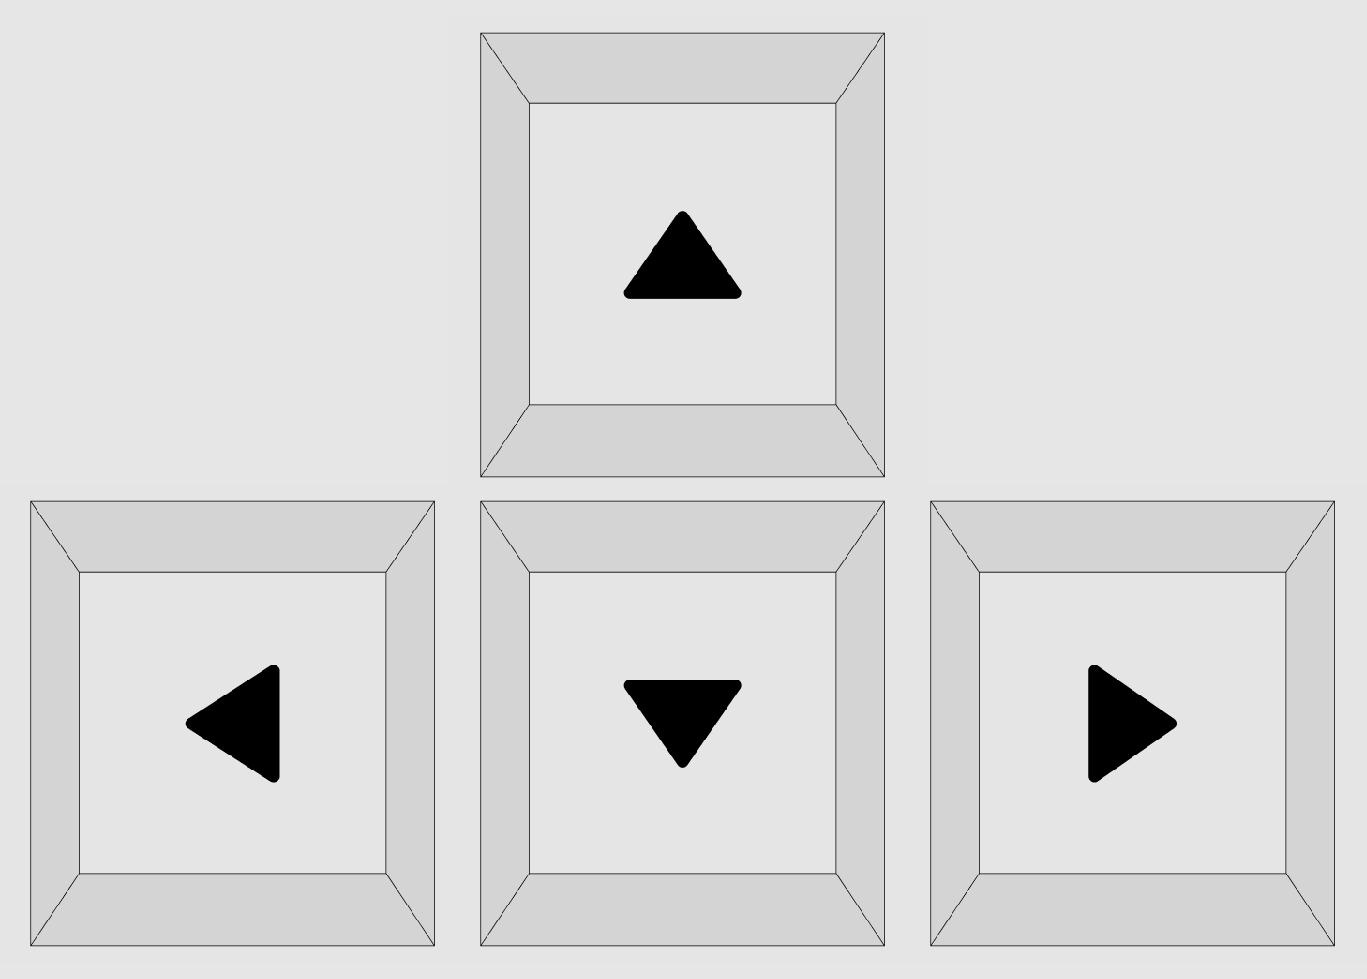
\includegraphics[height=3cm]{import/arrows.pdf}
	\end{center} 
	& Poruszanie kamerą na większych poziomach \\ 
	\hline 
	
	\begin{center}
		
\includegraphics[height=3cm]{import/mouse.pdf}
	\end{center}  & Pozostałe interakcje wykonywane przy pomocy myszki \\ 
	\hline
	

	\caption{Sterowanie}	
\end{longtable}
\end{center}

\subsubsection{Statystyki}
\begin{center}
\begin{longtable}{| p{.50\textwidth} | p{.50\textwidth} |} 
	\hline
	Health
	& Liczba punktów życia. Po utracie wszystkich punktów życia gracz przegrywa \\
	\hline
	Money
	& Złoto, które w danej chwili posiada użytkownik \\ 
	\hline 

	\caption{Statystyki gracza}	
\end{longtable}
\end{center}

\subsubsection{Interfejs użytkownika}

\begin{figure}[!htb]
	\begin{center}
		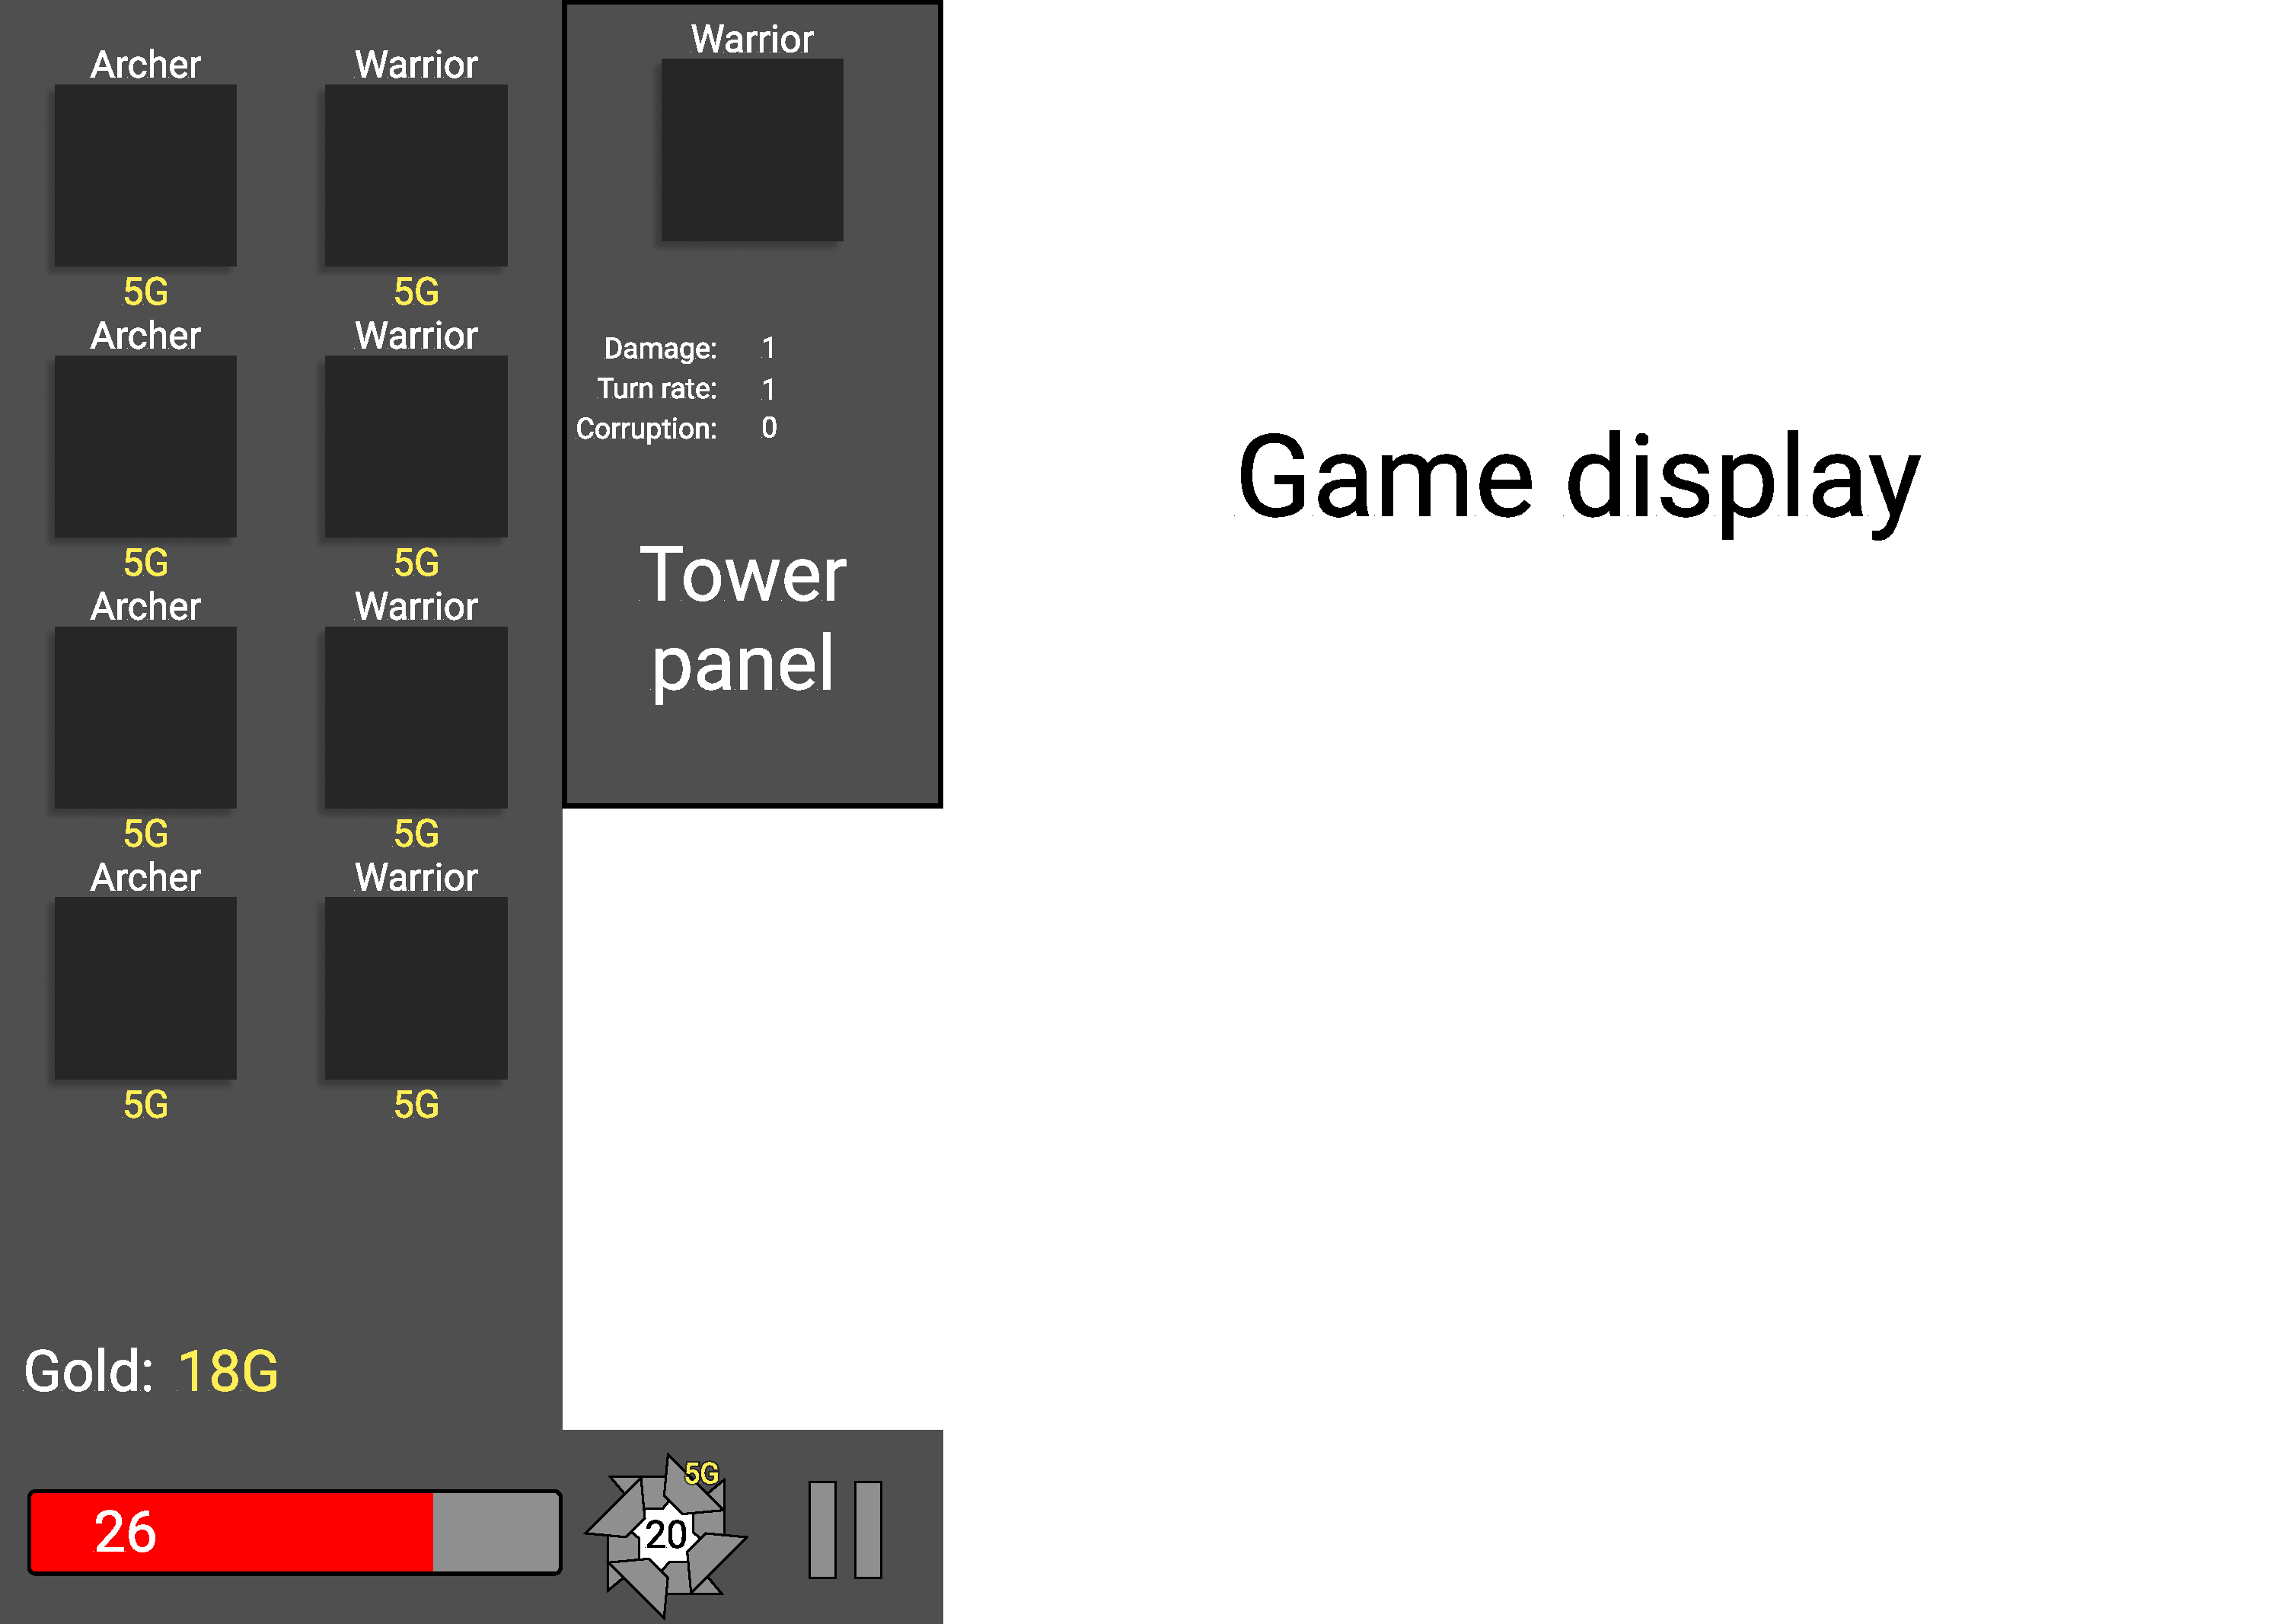
\includegraphics[width=12cm]{import/UI_Game.pdf}
	\end{center}
	\caption{UI w trakcje rozgrywki}
\end{figure}

Użytkownik z w trakcie rozgrywki widzi powyższy interfejs. W lewym dolnym rogu jest umieszczony pasek stanu życia gracza. Na prawo od tego elementu znajduje się wskaźnik czasu oraz przycisk zatrzymania rozgrywki w celu rozbudowy obrony. Przy wskaźniku czasu pojawia się liczba złota, którą otrzyma użytkownik gdy wymusi następną falę przeciwników. W tym celu należy nacisnąć na zegar. Nad paskiem życia znajduje się ilość złota jaką gracz aktualnie dysponuje.\\
Wyżej jest panel z dostępnymi wieżyczkami. Po wybraniu wieży z boku pojawia się panel z jej statystykami. W tym samym panelu widoczne są również statystyki wybranej wieży z pola bitwy. Taką wieżę można sprzedać i odzyskać część złota lub ulepszyć za pewną opłatą.
\newpage
\begin{figure}[!htb]
	\begin{center}
		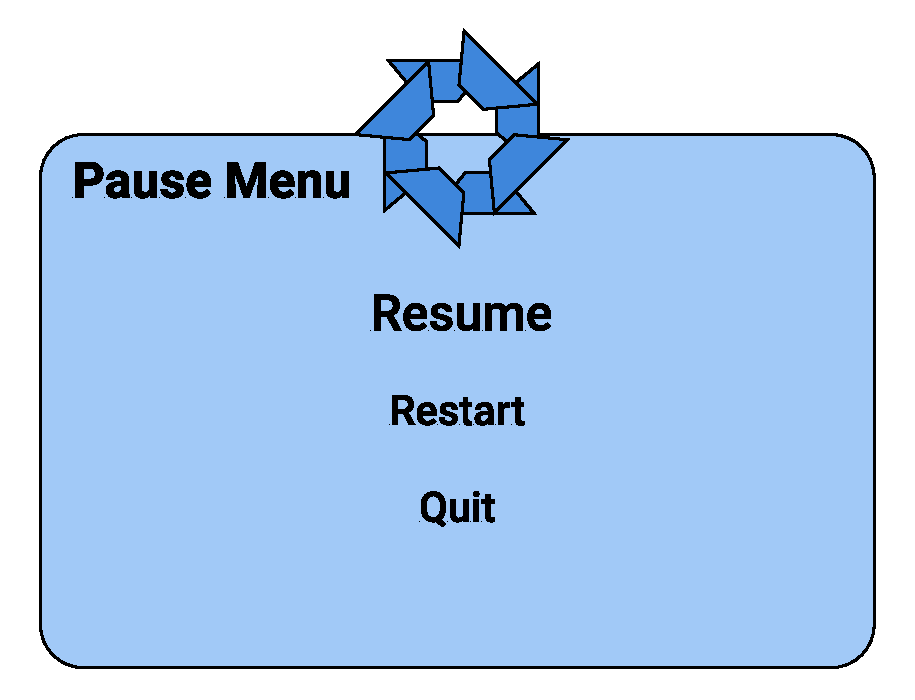
\includegraphics[width=7cm]{import/PauseMenu.pdf}
	\end{center}
	\caption{Menu pauzy}
\end{figure}

Za pomocą klawisza ESC lub po naciśnięciu odpowiedniego przycisku w interfejsie użytkownika, gracz może zatrzymać rozgrywkę. Otwiera się wtedy menu, za pomocą którego można powtórzyć poziom, powrócić do menu głównego lub kontynuować grę. Ponowne naciśnięcie ESC wznawia rozgrywkę.


\subsection{Przeciwnicy}
\subsubsection{Poruszanie}
Przeciwnicy poruszają się według wyznaczonej ścieżki na zasadzie punktów kontrolnych. Każdy typ przeciwnika ma swoją prędkość poruszania. W trakcie rozgrywki ta wartość może być modyfikowana przez efekty działania wież obronnych lub innych unikalnych przeciwników.
\subsubsection{Statystyki}
\begin{center}
\begin{longtable}{| p{.50\textwidth} | p{.50\textwidth} |} 
	\hline
	Health
	& Liczba punktów życia. Po utracie wszystkich punktów życuia przeciwnik ginie, a gracz otrzymuje złoto \\
	\hline
	Damage
	& Obrażenia jakie zostaną zadane graczowi, gdy przeciwnik dotrze do celu \\ 
	\hline 
	Defense
	& Odporność na obrażenia uwzględniana podczas obliczania obrażeń od wież \\ 
	\hline
	MovementSpeed
	& Szybkość poruszania się przeciwnika \\ 
	\hline
	GoldReward
	& Kwota otrzymywana po pokonaniu przeciwnika \\ 
	\hline

	\caption{Statystyki przeciwników}	
\end{longtable}
\end{center}

\subsubsection{Rodzaje przeciwników}
\begin{enumerate}
	\item Prehistoria
	\begin{itemize}
		\item Nieuzbrojony -- model postaci nie posiada żadnej broni, ubrany w prosty strój ze skóry.
		\begin{longtable}[l]{|c|c|} 
			\hline
			Health & 2 \\
			\hline
			Damage & 1 \\ 
			\hline 
			Defense & 0 \\ 
			\hline
			MovementSpeed & 5 \\ 
			\hline
			GoldReward & 1 \\ 
			\hline
		\end{longtable}
		
		\item Kamieniarz -- model postaci trzyma w ręku kamień wycięty na kształt noża, ubrany w prosty strój ze skóry, ale chroni większą część ciała niż w przypadku Nieuzbrojonego. Postać jest silniejsza, ale kosztem szybkości ruchu.
		\begin{longtable}[l]{|c|c|} 
			\hline
			Health & 4 \\
			\hline
			Damage & 3 \\ 
			\hline 
			Defense & 1 \\ 
			\hline
			MovementSpeed & 3 \\ 
			\hline
			GoldReward & 4 \\ 
			\hline
		\end{longtable}
	
		\item Procarz -- model postaci trzyma w ręku procę. Postać jest zwinniejsza od pozostałych, dlatego porusza się szybciej, ale łatwiej jest ją pokonać.
		\begin{longtable}[l]{|c|c|} 
			\hline
			Health & 1 \\
			\hline
			Damage & 1 \\ 
			\hline 
			Defense & 0 \\ 
			\hline
			MovementSpeed & 8 \\ 
			\hline
			GoldReward & 1 \\ 
			\hline
		\end{longtable}
		
	\end{itemize}
	
	\item Starożytność
	\begin{itemize} 
		\item Gladiator -- wojownik wyposażony w miecz i lekką zbroję.
		\begin{longtable}[l]{|c|c|} 
			\hline
			Health & 5 \\
			\hline
			Damage & 1 \\ 
			\hline 
			Defense & 0 \\ 
			\hline
			MovementSpeed & 6 \\ 
			\hline
			GoldReward & 4 \\ 
			\hline
		\end{longtable}
		
		\item Legionista -- postać wyposażona w miecz i prostokątną tarczę w pełnym pancerzu.
		\begin{longtable}[l]{|c|c|} 
			\hline
			Health & 7 \\
			\hline
			Damage & 3 \\ 
			\hline 
			Defense & 2 \\ 
			\hline
			MovementSpeed & 3 \\ 
			\hline
			GoldReward & 7 \\ 
			\hline
		\end{longtable}
		
		\item Rydwan -- pojazd ciągnięty przez konia. Jest szybki, ale można go łatwiej pokonać, ponieważ zarówno jeździeć jak i koń są narażeni na ataki.
		\begin{longtable}[l]{|c|c|} 
			\hline
			Health & 7 \\
			\hline
			Damage & 2 \\ 
			\hline 
			Defense & 1 \\ 
			\hline
			MovementSpeed & 11 \\ 
			\hline
			GoldReward & 9 \\ 
			\hline
		\end{longtable}
	\end{itemize}
	
	\item Średniowiecze
	\begin{itemize}
		\item Kmieć
		
		\item Rycerz
	
		\item Kawalerzysta
	\end{itemize}
\end{enumerate}

\subsection{Wieże}
Podstawowym elementem obrony gracza będą wieże umieszczane na wyznaczonych miejsca. Każda epoka historyczna ma unikatowe sposoby obrony. Wraz z postępem trybu kampanii, gracz będzie odblokowywał kolejne wieże.

\subsubsection{System celowania}
Gracz będzie miał możliwość wyboru systemu celowania, z którego w danej chwili ma korzystać każda wieża. Do wyboru będzie kilka opcji:
\begin{enumerate}
	\item Najbardziej oddalony cel -- obliczany jest dystans do każdego przeciwnika w zasięgi od wieży i wybierany jest najbardziej oddalony,
	\item Najbliższy cel -- obliczany jest dystans do każdego przeciwnika w zasięgu 
	\item Cel, który jest najbliżej bazy -- wybierany jest przeciwnik, który przebył największą odległość i jest w zasięgu strzału,
	\item Cel, który jest najdalej od bazy -- wybierany jest przeciwnik, który przebył najmnejszą odległość i jest w zasięgu strzału
	\item Losowy cel -- spośród przeciwników w zasięgu jest losowany jeden, który będzie atakowany. To jedyny tryb szukania przeciwników, który nie zmienia celu dopóki obecny cel wciąż żyje i jest w zasięgu.
\end{enumerate}

\subsubsection{Statystyki}

\begin{center}
\begin{longtable}{| p{.50\textwidth} | p{.50\textwidth} |} 
	\hline
	Range
	& Zasięg ataku wieży \\
	\hline
	Damage
	& Obrażenia, które otrzyma przeciwnik (zostaną zredukowane przez odporność przeciwnika) \\ 
	\hline 
	Corruption
	& Niszczenie pancerza, powoduje zmniejszenie odporności przeciwników \\ 
	\hline
	TurnRate
	& Szybkość obrotu \\ 
	\hline
	AttackSpeed
	& Częstotliwość ataków, szybkość ataku \\ 
	\hline
	BulletSpeed
	& Szybkość lotu pocisku \\ 
	\hline

	\caption{Statystyki wież}	
\end{longtable}
\end{center}

\subsubsection{Rodzaje wież}
\begin{enumerate}
	\item Prehistoria
	\begin{itemize}
		\item Kamieniarz -- postać rzuca kamieniami znalezionymi na ziemi.
		\begin{longtable}[l]{|c|c|} 
		\hline
		Range & 10 \\
		\hline
		Damage & 1 \\ 
		\hline 
		Corruption & 0 \\ 
		\hline
		TurnRate & 20 \\ 
		\hline
		AttackSpeed & 10 \\ 
		\hline
		BulletSpeed & 25 \\ 
		\hline
		\end{longtable}

		\item Procarz -- postać trzyma w ręku procę.
		\begin{longtable}[l]{|c|c|} 
		\hline
		Range & 15 \\
		\hline
		Damage & 2 \\ 
		\hline 
		Corruption & 0 \\ 
		\hline
		TurnRate & 20 \\ 
		\hline
		AttackSpeed & 7 \\ 
		\hline
		BulletSpeed & 40 \\ 
		\hline
		\end{longtable}		
		
		\item Włócznik -- postać rzuca naostrzonymi patykami
		\begin{longtable}[l]{|c|c|} 
		\hline
		Range & 8 \\
		\hline
		Damage & 2 \\ 
		\hline 
		Corruption & 1 \\ 
		\hline
		TurnRate & 15 \\ 
		\hline
		AttackSpeed & 4 \\ 
		\hline
		BulletSpeed & 30 \\ 
		\hline
		\end{longtable}	
	\end{itemize}
	
	\item Starożytność
	\begin{itemize}
		\item Rzucający nożem
		\begin{longtable}[l]{|c|c|} 
		\hline
		Range & 12 \\
		\hline
		Damage & 3 \\ 
		\hline 
		Corruption & 0 \\ 
		\hline
		TurnRate & 25 \\ 
		\hline
		AttackSpeed & 8 \\ 
		\hline
		BulletSpeed & 25 \\ 
		\hline
		\end{longtable}	
		
		\item Włócznik
		\begin{longtable}[l]{|c|c|} 
		\hline
		Range & 10 \\
		\hline
		Damage & 4 \\ 
		\hline 
		Corruption & 1 \\ 
		\hline
		TurnRate & 12 \\ 
		\hline
		AttackSpeed & 4 \\ 
		\hline
		BulletSpeed & 30 \\ 
		\hline
		\end{longtable}	
		\item Łucznik
		
	\end{itemize}

	\item Średniowiecze
	\begin{itemize}
		\item Łucznik -- postać wyposażona w łuk, na plecach ma założony kołczan
		\begin{longtable}[l]{|c|c|} 
		\hline
		Range & 12 \\
		\hline
		Damage & 3 \\ 
		\hline 
		Corruption & 0 \\ 
		\hline
		TurnRate & 18 \\ 
		\hline
		AttackSpeed & 10 \\ 
		\hline
		BulletSpeed & 30 \\ 
		\hline
		\end{longtable}	
		
		\item Kusznik
		\begin{longtable}[l]{|c|c|} 
		\hline
		Range & 20 \\
		\hline
		Damage & 4 \\ 
		\hline 
		Corruption & 2 \\ 
		\hline
		TurnRate & 15 \\ 
		\hline
		AttackSpeed & 5 \\ 
		\hline
		BulletSpeed & 50 \\ 
		\hline
		\end{longtable}		
	
		\item Katapulta
		\begin{longtable}[l]{|c|c|} 
		\hline
		Range & 25 \\
		\hline
		Damage & 8 \\ 
		\hline 
		Corruption & 0 \\ 
		\hline
		TurnRate & 10 \\ 
		\hline
		AttackSpeed & 3 \\ 
		\hline
		BulletSpeed & 40 \\ 
		\hline
		\end{longtable}	
	\end{itemize}
	
\end{enumerate} 
 
\section{Wnioski}
\begin{itemize}
	\item Projektowanie gier jest wymagającym zadaniem. Projektant musi mieć duże zdolności analityczne, ponieważ dobry projekt powinien być zupełny. Każdy aspekt gry musi być dobrze przemyślany, nie powinny występować elementy rozgrywki, które nie zostały przewidziane. Kolejnym aspektem dotyczącym projektowania jest balansowanie parametrami. W przypadku gry z gatunku "Tower Defense" należy odpowiednio dobrać statystyki przeciwników oraz wież, tak aby gra stanowiła wyzwanie dla gracza i zachęcała do dalszej rozgrywki. Zbyt wysoki lub zbyt niski poziom trudności może zniechęcić gracza.
	
	\item Unity3D to środowisko do tworzenia gier, ale również można w nim tworzyć różne animacje czy wizualizacje. Przy pierwszym uruchomieniu wydaje się dość skomplikowane ze względu na dużą liczbę okien. W rzeczywistości stosunkowo szybko można odnaleźć się w interfejsie. Dużą zaletą tego środowiska jest możliwość modyfikowania obiektów i ich parametrów przez zmiany wartości w interfejsie graficznym. Co więcej, każdy obiekt można dowolnie modyfikować poprzez dodanie do niego nowych skryptów -- własnych lub przygotowanych przez twórców. Dzięki temu każdy model może być wykorzystany wielokrotnie,a dostać zmienioną funkcjonalność poprzez podłączenie innych skryptów. Środowisko zapewnia bardzo dużo zróżnicowanych skryptów. Na przykład do paneli w interfejsie graficznym można dodać skrypty, które ustawią elementy potomne jeden pod drugim albo w innym przypadku w układzie siatki.
	
	\item Trzeba zwrócić uwagę na fakt, że implementacja gry wymaga umiejętności pracy w kilu dziedzinach. Po pierwsze potrzebne są skrypty, których przygotowanie bez wiedzy programistycznej byłoby bardzo trudne. Kolejny dział informatyki, bez którego tego typu gra nie powstanie to grafika komputerowa. Należy przygotować modele, interfejs graficzny, to są elementy, które są widoczne dla gracza. Skrypty są ukryte przed graczem, widzi je pośrednio przez zachowanie poszczególnych modeli. Warto też wspomnieć o muzyce, która również wpływa na nastawienie gracza. Podsumowując, tworzenie gry przez jedną osobę jest bardzo wymagające, jeżeli chce się zadbać o każdy z wymienionych aspektów.
	
	\item Dokumentacja dla Unity3D jest bardzo rozbudowana. Dotyczy to samego środowiska oraz ScriptingAPI. Unity opracowało przyjemną możliwość pisania skryptów. Klasy, które są skryptami rozszerzają interfejs MonoBehaviour. Skrypty mają ustaloną kolejność wykonywania funkcji.  Kiedy na scenie pojawia się obiekt z konkrentym skryptem, to w tym skrypcie wykonuje się w pierwszej kolejności metoda Awake, w której inicjalizuje się parametry, które powinny zostać stworzone w pierwszej kolejności. Na przykład w stworzonej grze w tej metodzie ustalane są kolejne punkty po których poruszają się przeciwnicy, żeby później przekazać ja do elementu, który zarządza pojawianiem się przeciwników. Pozostałe inicjalizacje wykonywane są w metodzie Start. Dzięki temu powstaje swego rodzaju hierarchia wykonywania poszczególnych elementów. Metoda Update służy jako nieskończona pętla, dzięki której obiekt może wykonywać jakieś akcje (na przykład poruszanie się). Ze względu na zmienną liczbę klatek na sekundę w grach, często wykorzystuje się Time.deltaTime, która daje informacje ile czasu upłynęło pomiedzy poszczególnymi klatkami. Pozwala to płynne działanie gry.
	
	\item Przechodząc do etapu programowania, tworzenia gry, zdarza się, że pewne pomysły ulegają modyfikacjom, usprawnieniom. Jest to ważny element rozwoju oprogramowania, ponieważ dopiero jak zaczniemy pracę nad projektem, to zaczynamy dostrzegać pewne niedoskonałości, które warto jest poprawić. W przypadku mojego projektu modyfikacjom ulegał system ścieżki poruszania się przeciwników. W początkowej wersji przygotowałem globalną drogę, z której korzystał każdy obiekt tworzący przeciwników (nawet jeżeli znajdowały się w zupełnie innych miejscach na planszy). Zdecydowałem się to zmienić, każdy obiekt pojawiający ma teraz przypisaną własną ścieżkę, dzięki czemu można tworzyć bardziej złożone poziomy. Mimo, że rozwiązanie jest skuteczne, to trzeba każdemu obiektowi wyznaczyć tę ścieżkę, dlatego rozważam przygotowanie dwuwymiarowej przestrzeni, na której ścieżki będą przypominały labirynt, natomiast skrypt zamiast otrzymywać gotową ścieżkę będzie ją wyszukiwał. Zakładam możliwość użycia algorytmu A*, DFS, albo BFS. Stąd wniosek, że oprogramowanie nie jest czymś stałym, niezmiennym. Dobre oprogramowanie to takie, które ciągle się rozwija, usprawnia poszczególne elementy, o ile to możliwe.
\end{itemize}
 
\newpage
\section{Bibliografia}

\begingroup
\renewcommand{\section}[2]{}%
\begin{thebibliography}{}
\bibitem{GDD-stanley}
	Alec Markarian, Benjamin Stanley.
	\emph{Game Design Document}

	\href{https://docs.google.com/document/d/1-I08qX76DgSFyN1ByIGtPuqXh7bVKraHcNIA25tpAzE}{docs.google.com/document/d/1-I08qX76DgSFyN1ByIGtPuqXh7bVKraHcNIA25tpAzE}\\
	(dostęp 29.02.2020)

\bibitem{GDD}
	Chop Socky Chooks in Bantam Menace Game Design Document Version 1.1 Gas Ferry Rd, Bristol, BS1 6UN, \url{http://www.photonstorm.com/downloads/CSC_GDD.pdf}\\
	(dostęp 29.02.2020)

\end{thebibliography}
\endgroup

\end{document}

